% Provenance (never printed): old premiere S material on subduction (Wadati-Benioff
% planes, density of the old lithosphere, slab pull, transformation of the slab at
% depth: blueschist and eclogite; anatomy of an active margin). Sections from
% figdata/grade-11/slab_sections.py (USGS ComCat M >= 6 1976-2025, PB2002 steps,
% Seton 2020 ages); plate speeds from plate_velocities.py (NNR-MORVEL56 RMS).
% Metamorphism is defined in g12.03, the volcanic arc in g12.04: named only here.
\chapter{Zona Subduksi}\label{ch:g11:subduction-zones}

Di bawah Kepulauan Tonga, di Pasifik barat daya, Bumi berguncang jauh lebih
dalam daripada di tempat lain mana pun. Dari tujuh ribu gempa bumi bermagnitudo
6 atau lebih yang tercatat di seluruh dunia antara tahun 1976 dan 2025, yang
paling dalam terjadi pada kedalaman \qty{688}{km}, dan penampang melintasi Tonga
dalam bab ini memuat peristiwa sampai kedalaman sekitar \qty{671}{km}. Pada
kedalaman seperti itu batuan panas dan berada di bawah tekanan yang sangat besar;
batuan itu seharusnya mengalir perlahan, seperti \omterm{def:g11:lithosphere-asthenosphere:lithosphere}{astenosfer}, bukan patah. Namun
batuan itu patah. Bab ini menjelaskan apa yang ada di sana untuk patah: sebuah
\omterm{def:g11:subduction-zones:slab}{lempengan} dasar samudra yang dingin, yang tenggelam kembali ke dalam mantel.
% ledger: data:usgs-comcat (catalogue_maxdepth 688; tonga_maxdepth 670.8, slab_sections.py)

\begin{recall}
Di batas konvergen dua lempeng bergerak saling mendekat; palung-palung dalam
membatasi sebagian di antaranya (Buku 1, kelas 7 dan 8). Magnitudo gempa bumi
mengukur besarnya, dan gempa bumi di bawah laut dapat membangkitkan tsunami
(Buku 1, kelas 7). Kecepatan sebuah lempeng relatif terhadap lempeng lain adalah
selisih kecepatan keduanya (\cref{ch:g11:plate-motions}). Dasar samudra tenggelam
seiring umurnya, dan setelah sekitar 60 juta tahun \omterm{def:g11:lithosphere-asthenosphere:lithosphere}{litosfernya}, yang setebal
sekitar \qty{100}{km}, lebih rapat daripada \omterm{def:g11:lithosphere-asthenosphere:lithosphere}{astenosfer} di bawahnya
(\cref{ch:g11:ocean-ridges}). Gelombang seismik menunjukkan perubahan yang tajam
di mantel pada sekitar \qty{670}{km} (\cref{ch:g11:seismic-structure}). Batuan
metamorf adalah batuan yang berubah dalam keadaan padat (Buku 1, kelas 6).
\end{recall}
% ledger: data:prem (670 km), ps77:depth-age

\section{Palung dan zona gempa bumi yang miring}

Kebanyakan gempa bumi dangkal: dalam katalog gempa bumi bermagnitudo 6 atau lebih
sejak 1976, hanya sekitar satu dari lima yang lebih dalam daripada \qty{70}{km},
dan satu dari lima belas yang lebih dalam daripada \qty{300}{km}. Peta di bawah
menunjukkan letak gempa-gempa bumi yang dalam itu.
% values (slab_sections.py): frac_deeper_70 0.21, frac_deeper_300 0.069; data:usgs-comcat

\begin{omfigure}
\begin{tikzpicture}
\begin{axis}[ommap, width=\linewidth, xtick={-180,-90,...,180}, ytick={-60,0,60},
  legend style={font=\scriptsize, at={(0.5,-0.13)}, anchor=north, legend columns=3,
    /tikz/every even column/.append style={column sep=6pt}}]
\addplot[fill=omLithAlluv, draw=black!45, line width=0.2pt, forget plot] table {figdata/out/shared-geo-land.dat};
\addplot[black!70, line width=0.5pt, forget plot] table {figdata/out/shared-geo-school-subduction.dat};
\addplot[fill=black!70, draw=none, forget plot] table {figdata/out/shared-geo-school-teeth.dat};
% computed in figdata/grade-11/slab_sections.py; ledger: data:usgs-comcat, data:pb2002
\addplot[only marks, mark=*, mark size=0.55pt, black!45] table[x=lon, y=lat] {figdata/out/grade-11-slab_sections-world-shallow.dat};
\addplot[only marks, mark=*, mark size=0.8pt, omProp] table[x=lon, y=lat] {figdata/out/grade-11-slab_sections-world-mid.dat};
\addplot[only marks, mark=*, mark size=1.1pt, omThm] table[x=lon, y=lat] {figdata/out/grade-11-slab_sections-world-deep.dat};
\legend{{lebih dangkal daripada \qty{70}{km}}, {70 sampai \qty{300}{km}}, {lebih dalam daripada \qty{300}{km}}}
\end{axis}
\end{tikzpicture}

{\small Gempa bumi bermagnitudo 6.5 atau lebih, 1976--2025 (2192 peristiwa),
diwarnai menurut kedalamannya, dengan palung-palung (garis hitam, segitiga pada
lempeng yang berada di atas). Gempa bumi menengah dan dalam hanya terletak di
sepanjang sebagian palung, selalu di sisi lempeng yang berada di atas. Data:
katalog gempa bumi USGS; batas lempeng dari Bird (2003); daratan dari Natural
Earth.}
\end{omfigure}
% values: world_n_m65 2192, world_deep_n 197 (slab_sections.py)

Gempa bumi yang dalam tidak tersebar acak: gempa-gempa itu mengikuti palung-palung
di Pasifik barat, dari Kamchatka ke Jepang, Kepulauan Mariana, Indonesia, dan
Tonga, dan palung di sepanjang pantai barat Amerika Selatan; dan gempa-gempa itu
selalu terletak di satu sisi palung, di bawah lempeng yang tidak tenggelam.

\begin{definition}[Subduksi; zona subduksi]\label{def:g11:subduction-zones:subduction}
Yang disebut \emph{subduksi}\index{subduksi} adalah tenggelamnya lempeng
\omterm{def:g11:ocean-ridges:oceanic-lithosphere}{litosfer samudra} di bawah lempeng lain, kembali ke dalam mantel. Yang disebut
\emph{zona subduksi}\index{zona subduksi} adalah batas lempeng konvergen tempat
subduksi berlangsung; di permukaan zona itu ditandai oleh palung.
\end{definition}

\begin{definition}[Zona Wadati--Benioff]\label{def:g11:subduction-zones:benioff}
Yang disebut \emph{zona Wadati--Benioff}\index{zona Wadati--Benioff} adalah pita
gempa bumi yang miring yang bermula di palung dan makin lama makin dalam di
bawah lempeng yang berada di atas, sampai sedalam sekitar \qty{700}{km}.
\end{definition}
% ledger: frohlich87:wadati

\begin{history}[Wadati dan Benioff]
Pada tahun 1920-an para ahli seismologi terkemuka berpendapat bahwa gempa bumi
hanya dapat terjadi pada beberapa puluh kilometer pertama: menurut penalaran
mereka, bagian Bumi yang lebih dalam tidak mempunyai kekuatan untuk menyimpan
regangan. Ahli seismologi Jepang Kiyoo Wadati, yang bekerja dengan jaringan
stasiun yang rapat milik Badan Meteorologi Jepang, memberikan sejak tahun 1928
bukti pertama yang meyakinkan bahwa sebagian gempa bumi terjadi ratusan kilometer
di bawah permukaan: salah satu peristiwa yang dipelajarinya, pada bulan Januari
1927, terjadi pada kedalaman \qty{420}{km}. Pada tahun 1935 ia menerbitkan peta
pertama kedalaman gempa-gempa bumi itu, yang digambar sebagai garis kontur, dan
memperhatikan bahwa zona yang makin dalam itu sejajar dengan deretan gunung api
aktif. Pada tahun 1949 dan 1954 ahli seismologi Amerika Hugo Benioff menunjukkan
bahwa di bawah Andes dan Kepulauan Tonga--Kermadec gempa-gempa bumi terletak di
sepanjang zona yang mencapai kedalaman sekitar \qty{700}{km}. Zona-zona itu
mula-mula disebut zona Benioff, pada tahun 1967; nama \omterm{def:g11:subduction-zones:benioff}{zona Wadati--Benioff}, yang
menghargai jasa keduanya, berasal dari usul yang diajukan oleh ahli geofisika
Jepang Seiya Uyeda pada tahun 1971.
\end{history}
% ledger: frohlich87:wadati

\begin{method}[Membaca penampang gempa bumi]\label{met:g11:subduction-zones:section}
\begin{enumerate}
  \item Pilih sebuah garis yang tegak lurus pada palung, dari palung ke arah
        lempeng yang berada di atas, dan ambil gempa-gempa bumi di dalam
        sebuah pita di kedua sisinya.
  \item Gambarkan setiap gempa bumi pada jaraknya di sepanjang garis itu
        (mendatar) dan pada kedalamannya (tegak, ke bawah).
  \item Cari pita yang miring; tarik garis lurus yang paling baik
        mengikutinya.
  \item Baca kemiringan pita itu dari dua titik pada garis tersebut (proposisi
        di bawah).
\end{enumerate}
\end{method}

\begin{omfigure}
\begin{tikzpicture}
\begin{axis}[omrecord, omdepth, name=tonga, width=0.5\linewidth, height=6.4cm,
  xmin=-150, xmax=900, ymin=0, ymax=720, xlabel={jarak dari palung (\unit{km})},
  ylabel={kedalaman (\unit{km})}, title={\small Tonga}, clip=false]
% computed in figdata/grade-11/slab_sections.py; ledger: data:usgs-comcat, data:pb2002
\addplot[only marks, mark=*, mark size=1.2pt, black!65] table[x=x, y=depth] {figdata/out/grade-11-slab_sections-tonga.dat};
\addplot[omProp, line width=1pt, domain=135.7:761.6, samples=2] {-23.568 + 0.91068*x};
\addplot[only marks, mark=triangle*, mark size=3pt, omDef] coordinates {(0,0)};
\node[font=\scriptsize, anchor=south west, text=omDef] at (axis cs:10,8) {palung};
\node[font=\scriptsize, anchor=west, text=omProp, align=left] at (axis cs:300,560) {kemiringan\\\ang{42}};
\end{axis}
\begin{axis}[omrecord, omdepth, at={(tonga.east)}, anchor=west, xshift=0.3cm, width=0.5\linewidth, height=6.4cm,
  xmin=-150, xmax=900, ymin=0, ymax=720, xlabel={jarak dari palung (\unit{km})},
  yticklabels={}, title={\small Andes, dekat \ang{21} LS}, clip=false]
\addplot[only marks, mark=*, mark size=1.2pt, black!65] table[x=x, y=depth] {figdata/out/grade-11-slab_sections-andes.dat};
\addplot[omProp, line width=1pt, domain=253.0:900, samples=2] {-88.745 + 0.74613*x};
\addplot[only marks, mark=triangle*, mark size=3pt, omDef] coordinates {(0,0)};
\node[font=\scriptsize, anchor=south west, text=omDef] at (axis cs:10,8) {palung};
\node[font=\scriptsize, anchor=west, text=omProp, align=left] at (axis cs:300,560) {kemiringan\\\ang{37}};
\end{axis}
\end{tikzpicture}

{\small Penampang gempa bumi yang tegak lurus pada dua palung: gempa bumi
bermagnitudo 6 atau lebih, 1976--2025, dalam jarak \qty{150}{km} dari garis
penampang, yang digambarkan pada jaraknya dari palung (ke arah lempeng yang
berada di atas) dan kedalamannya. Jingga: garis lurus yang paling baik mengikuti
gempa-gempa bumi pada kedalaman antara 100 dan \qty{600}{km}. Di bawah Tonga
pita itu mencapai lebih dalam daripada \qty{670}{km}. Data: katalog gempa bumi
USGS; posisi palung dari Bird (2003).}
\end{omfigure}
% values (slab_sections.py): tonga_dip 42.3, fit -23.568 + 0.91068 x (77 events);
% andes_dip 36.7, fit -88.745 + 0.74613 x; trench points tonga (-173.31, -20.395),
% andes (-71.286, -21.01)

\begin{proposition}[Kemiringan lempengan dari penampang gempa bumi]\label{prop:g11:subduction-zones:dip}
Jika dua titik pada garis yang mengikuti \omterm{def:g11:subduction-zones:benioff}{zona Wadati--Benioff} terletak pada
jarak mendatar $x_1 < x_2$ dari palung dan pada kedalaman $z_1$ dan $z_2$,
kemiringannya $\delta$, yaitu sudut yang dibentuknya dengan bidang datar, memenuhi
\[
  \tan \delta = \frac{z_2 - z_1}{x_2 - x_1}.
\]
\end{proposition}

\begin{proof}
Kedua titik itu dan titik pada kedalaman $z_1$ tegak lurus di atas titik kedua
membentuk segitiga siku-siku. Sisi mendatarnya $x_2 - x_1$, sisi tegaknya
$z_2 - z_1$, dan sudut di titik pertama adalah kemiringannya. Tangen suatu sudut
dalam segitiga siku-siku adalah sisi di depan sudut itu dibagi sisi di
sampingnya.
\end{proof}

\begin{example}[Kemiringan di bawah Tonga]\label{ex:g11:subduction-zones:dip}
Garis penampang Tonga melalui kedalaman \qty{250}{km} pada jarak \qty{300}{km}
dari palung dan kedalaman \qty{614}{km} pada jarak \qty{700}{km}. Jadi
$\tan\delta = (614 - 250)/(700 - 300) = 364/400 = 0.91$, dan
$\delta \approx \ang{42}$. Di bawah Andes, pada \ang{21}~LS, metode yang sama
memberikan sekitar \ang{37}.
\end{example}
% values: tonga line at 300 km 249.6, at 700 km 613.9 (slab_sections.py)

\omterm{def:g11:subduction-zones:benioff}{Zona Wadati--Benioff} menelusuri lempeng yang turun. Gempa bumi dangkal terjadi
di tempat kedua lempeng saling bergeser, di dekat palung; gempa bumi yang lebih
dalam terjadi di dalam lempeng yang tenggelam itu sendiri.

\section{Mengapa litosfer tua tenggelam}

\begin{definition}[Lempengan]\label{def:g11:subduction-zones:slab}
Yang disebut \emph{lempengan}\index{lempengan} adalah bagian lempeng yang telah
tenggelam ke dalam mantel di \omterm{def:g11:subduction-zones:subduction}{zona subduksi}: selembar \omterm{def:g11:ocean-ridges:oceanic-lithosphere}{litosfer samudra}, setebal
sekitar seratus kilometer, yang miring di bawah lempeng yang berada di atas.
\end{definition}

Yang turun adalah dasar samudra yang tua. Menurut umur dasar samudra, dasar yang
mencapai Palung Jepang, di timur Jepang, berumur sekitar 133 juta tahun, dasar
yang mencapai Palung Tonga sekitar 99 juta tahun; bahkan dasar yang mencapai
Andes, salah satu yang termuda yang tenggelam, berumur sekitar 49 juta tahun.
\omterm{def:g11:lithosphere-asthenosphere:lithosphere}{Litosfer} setua itu dingin dan tebal, dan, kecuali keraknya yang ringan, lebih
rapat daripada \omterm{def:g11:lithosphere-asthenosphere:lithosphere}{astenosfer}: begitu salah satu tepinya mulai turun, beratnya
sendiri menariknya masuk.
% values (slab_sections.py): japan_age 133.1, tonga_age 98.8, andes_age 48.8 (median of the
% 1-degree cells 100-400 km seaward of the trench point); ledger data:b2-seafloor-age

\begin{definition}[Tarikan lempengan; dorongan punggung]\label{def:g11:subduction-zones:slab-pull}
Yang disebut \emph{tarikan lempengan}\index{tarikan lempengan} adalah gaya yang
dikerjakan \omterm{def:g11:subduction-zones:slab}{lempengan} yang tenggelam, yang lebih rapat daripada mantel di
sekitarnya, pada bagian lain lempengnya, yang menariknya ke arah palung. Yang
disebut \emph{dorongan punggung}\index{dorongan punggung} adalah gaya yang
mendorong lempeng menjauhi punggung samudra, tempat \omterm{def:g11:lithosphere-asthenosphere:lithosphere}{litosfer} yang muda dan panas
berdiri tinggi di atas punggungnya yang terangkat dan meluncur menuruni lerengnya.
\end{definition}

Manakah di antara keduanya yang lebih penting? Pada tahun 1975 Donald Forsyth dan
Seiya Uyeda menghitung kekuatan setiap gaya dari kecepatan dan bentuk
lempeng-lempeng: gaya-gaya pada \omterm{def:g11:subduction-zones:slab}{lempengan} yang tenggelam mengendalikan kecepatan
lempeng-lempeng samudra, dan sekitar sepuluh kali lebih kuat daripada gaya lain
mana pun. Kecepatan lempeng masa kini menunjukkannya dengan jelas.
% ledger: fu75:slab-pull

\begin{omfigure}
\begin{tikzpicture}
\begin{axis}[omrecord, ybar, bar width=9pt, width=0.86\linewidth, height=5.6cm,
  ymin=0, ymax=85, xmin=-0.7, xmax=12.7, bar shift=0pt, ylabel={kecepatan rata-rata (\unit{mm} setahun)},
  xtick={0,...,12}, xticklabel style={rotate=50, anchor=east, font=\scriptsize},
  xticklabels={Cocos, Nazca, Pasifik, Australia, Laut Filipina, Arab, Somalia,
    Nubia, Eurasia, Amerika Utara, Antarktika, Karibia, Amerika Selatan},
  ymajorgrids, xmajorgrids=false]
% computed in figdata/grade-11/slab_sections.py from plate_velocities.POLES (nnr56:rms)
\addplot[fill=omProp, draw=omProp!70!black] table[x=idx, y expr=\thisrow{slab}*\thisrow{rms}] {figdata/out/grade-11-slab_sections-speeds.dat};
\addplot[fill=omDef!35, draw=omDef] table[x=idx, y expr=(1-\thisrow{slab})*\thisrow{rms}] {figdata/out/grade-11-slab_sections-speeds.dat};
\node[font=\scriptsize, text=omProp!80!black, anchor=south] at (axis cs:2,76) {lempengan tergantung pada lempeng};
\node[font=\scriptsize, text=omDef, anchor=south] at (axis cs:9,50) {tanpa lempengan panjang};
\end{axis}
\end{tikzpicture}

{\small Kecepatan rata-rata tiga belas lempeng besar (akar rata-rata kuadrat atas
lempeng, dalam kerangka acuan yang di dalamnya \omterm{def:g11:lithosphere-asthenosphere:lithosphere}{litosfer} secara keseluruhan tidak
berputar). Jingga: lempeng yang padanya \omterm{def:g11:subduction-zones:slab}{lempengan} yang tenggelam tergantung di
sepanjang tepi yang panjang; biru: lempeng tanpa \omterm{def:g11:subduction-zones:slab}{lempengan} seperti itu. India
tidak disertakan: tepi utaranya adalah zona tumbukan. Data: NNR-MORVEL56 (Argus,
Gordon, dan DeMets, 2011).}
\end{omfigure}
% ledger: nnr56:rms; the bars of a class are drawn at 0 for the other (two series on one axis)

\begin{proposition}[Lempeng yang terikat pada lempengan bergerak cepat]\label{prop:g11:subduction-zones:fast}
Kelima lempeng besar yang padanya tergantung \omterm{def:g11:subduction-zones:slab}{lempengan} panjang (Cocos, Nazca,
Pasifik, Australia, Laut Filipina) bergerak rata-rata sekitar \qty{65}{mm}
setahun; delapan lempeng yang tidak mempunyainya sekitar \qty{24}{mm} setahun,
hampir tiga kali lebih lambat. Setiap lempeng dalam kelompok pertama lebih cepat
daripada setiap lempeng dalam kelompok kedua.
\end{proposition}
% values: rms_slab_mean 65.2, rms_noslab_mean 23.9 (plate_velocities.py); India left out
% (its northern edge is a collision)

\begin{proof}
Dari kecepatan rata-rata yang diterbitkan, lempeng-lempeng berlempengan memberikan
$(74.6 + 70.0 + 65.5 + 63.1 + 52.6)/5 \approx 65.2$ dan lempeng-lempeng lainnya
$(47.6 + 31.0 + 29.2 + 22.8 + 19.8 + 15.2 + 14.9 + 10.6)/8 \approx 23.9$
(milimeter setahun); lempeng berlempengan yang paling lambat, lempeng Laut
Filipina dengan 52.6, lebih cepat daripada lempeng lain yang paling cepat, Arab
dengan 47.6.
\end{proof}
% ledger: nnr56:rms

\section{Lempengan yang berubah di kedalaman}

Ketika \omterm{def:g11:subduction-zones:slab}{lempengan} turun, keraknya yang terdiri atas basalt dan \omterm{def:g11:ocean-ridges:gabbro}{gabro} terkubur makin
dalam sambil tetap dingin, karena \omterm{def:g11:subduction-zones:slab}{lempengan} tenggelam lebih cepat daripada
kecepatan kalor mencapai bagian dalamnya. Batuan kerak mengubah mineral-mineralnya
tanpa meleleh: batuan itu termetamorfosis (\cref{ch:g12:metamorphic-rocks}). Dua
batuan menandai lintasannya.

\begin{definition}[Sekis biru; eklogit]\label{def:g11:subduction-zones:eclogite}
Yang disebut \emph{sekis biru}\index{sekis biru} adalah batuan metamorf yang
terbentuk dari basalt \omterm{def:g11:ocean-ridges:oceanic-lithosphere}{kerak samudra} yang terkubur sampai bertekanan tinggi
sementara tetap relatif dingin; batuan ini diwarnai biru oleh mineral glaukofan.
Yang disebut \emph{eklogit}\index{eklogit} adalah batuan metamorf yang rapat yang
terbentuk dari basalt dan \omterm{def:g11:ocean-ridges:gabbro}{gabro} pada kedalaman mantel di sepanjang \omterm{def:g11:subduction-zones:subduction}{zona subduksi}:
komposisi kimianya sama, tetapi batuan ini terdiri atas garnet merah dan piroksen
hijau.
\end{definition}
% ledger: photo:g11-blueschist, photo:g11-eclogite

\begin{omfigure}
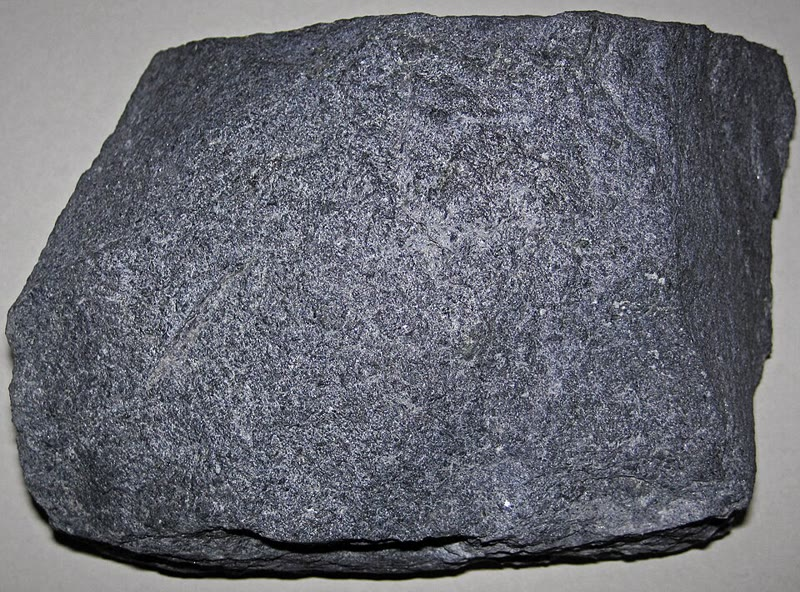
\includegraphics[height=4.4cm]{images/book2/g11-stjohn-blueschist.jpg}\hspace{0.03\linewidth}%
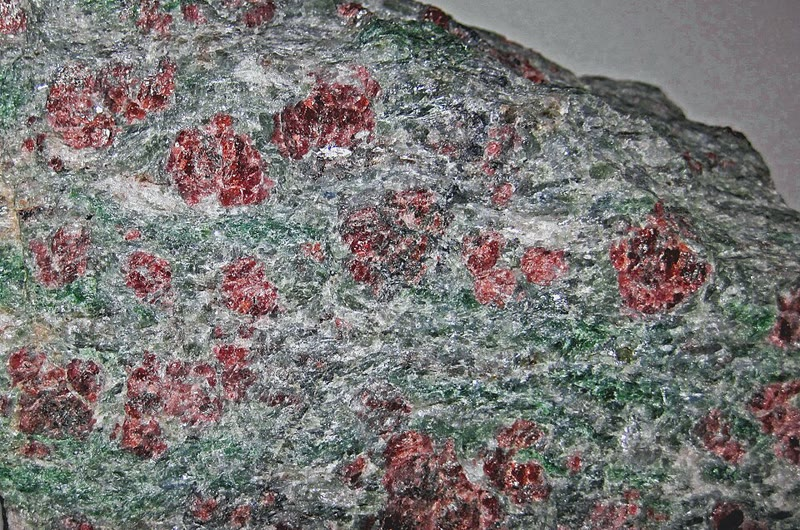
\includegraphics[height=4.4cm]{images/book2/g11-stjohn-eclogite.jpg}

{\small Kiri: \omterm{def:g11:subduction-zones:eclogite}{sekis biru} dari Pulau Santa Catalina, California, yang dahulu
merupakan \omterm{def:g11:ocean-ridges:oceanic-lithosphere}{kerak samudra} yang terkubur di \omterm{def:g11:subduction-zones:subduction}{zona subduksi}. Kanan: \omterm{def:g11:subduction-zones:eclogite}{eklogit} dari
Norwegia, dengan garnet merah di dalam piroksen hijau. Foto James St.~John
(CC~BY~2.0).}
\end{omfigure}
% ledger: photo:g11-blueschist, photo:g11-eclogite

\omterm{def:g11:subduction-zones:eclogite}{Eklogit} lebih rapat daripada basalt; \omterm{def:g11:subduction-zones:eclogite}{eklogit} bahkan lebih rapat daripada
\omterm{def:g11:ocean-ridges:peridotite}{peridotit} mantel, sekitar \qty{6}{\percent}. Begitu keraknya berubah menjadi
\omterm{def:g11:subduction-zones:eclogite}{eklogit}, \omterm{def:g11:subduction-zones:slab}{lempengan} tidak lagi membawa lapisan ringan di atasnya: seluruh
\omterm{def:g11:subduction-zones:slab}{lempengan} lebih rapat daripada mantel di sekitarnya, dan menarik lebih kuat.
Batuan semacam ini, yang dibawa kembali ke permukaan oleh gerakan-gerakan
kemudian, termasuk segelintir saksi langsung tentang apa yang terjadi puluhan
kilometer di bawah permukaan di \omterm{def:g11:subduction-zones:subduction}{zona subduksi}.
% ledger: hacker03:eclogite, photo:g11-eclogite

\begin{omfigure}
\begin{tikzpicture}[font=\footnotesize, scale=0.85]
  % subduction zone, a drawing, not to scale: slab top flat to x = -1, then bends to a 42-degree dip
  % coordinates computed once by a small script (scratch, not kept): slab top flat to x=-1, arc R=3 to a 42-degree dip
  \fill[omProp!10] (-7,-1.4) rectangle (7,-6.0);
  \fill[omSea!45] (-7,0) -- (-1,0) -- (1.6,0.8) -- (-7,0.8) -- cycle;
  \fill[lith peridotite] (-7.000,0.000) -- (-6.644,0.000) -- (-6.289,0.000) -- (-5.933,0.000) -- (-5.578,0.000) -- (-5.222,0.000) -- (-4.867,0.000) -- (-4.511,0.000) -- (-4.156,0.000) -- (-3.800,0.000) -- (-3.445,0.000) -- (-3.089,0.000) -- (-2.734,0.000) -- (-2.378,0.000) -- (-2.023,0.000) -- (-1.667,0.000) -- (-1.312,0.000) -- (-0.956,-0.000) -- (-0.602,-0.027) -- (-0.253,-0.094) -- (0.085,-0.203) -- (0.408,-0.351) -- (0.712,-0.536) -- (0.991,-0.756) -- (1.255,-0.994) -- (1.519,-1.232) -- (1.784,-1.470) -- (2.048,-1.707) -- (2.312,-1.945) -- (2.576,-2.183) -- (2.840,-2.421) -- (3.105,-2.659) -- (3.369,-2.897) -- (3.633,-3.135) -- (3.897,-3.373) -- (4.161,-3.611) -- (4.426,-3.848) -- (4.690,-4.086) -- (4.954,-4.324) -- (5.218,-4.562) -- (5.483,-4.800) -- (4.546,-5.840) -- (4.282,-5.603) -- (4.017,-5.365) -- (3.753,-5.127) -- (3.489,-4.889) -- (3.225,-4.651) -- (2.961,-4.413) -- (2.696,-4.175) -- (2.432,-3.937) -- (2.168,-3.699) -- (1.904,-3.461) -- (1.639,-3.224) -- (1.375,-2.986) -- (1.111,-2.748) -- (0.847,-2.510) -- (0.583,-2.272) -- (0.318,-2.034) -- (0.062,-1.803) -- (-0.087,-1.686) -- (-0.249,-1.587) -- (-0.421,-1.508) -- (-0.602,-1.450) -- (-0.788,-1.414) -- (-0.977,-1.400) -- (-1.312,-1.400) -- (-1.667,-1.400) -- (-2.023,-1.400) -- (-2.378,-1.400) -- (-2.734,-1.400) -- (-3.089,-1.400) -- (-3.445,-1.400) -- (-3.800,-1.400) -- (-4.156,-1.400) -- (-4.511,-1.400) -- (-4.867,-1.400) -- (-5.222,-1.400) -- (-5.578,-1.400) -- (-5.933,-1.400) -- (-6.289,-1.400) -- (-6.644,-1.400) -- (-7.000,-1.400) -- cycle;
  \fill[lith basalt] (-7.000,0.000) -- (-6.644,0.000) -- (-6.289,0.000) -- (-5.933,0.000) -- (-5.578,0.000) -- (-5.222,0.000) -- (-4.867,0.000) -- (-4.511,0.000) -- (-4.156,0.000) -- (-3.800,0.000) -- (-3.445,0.000) -- (-3.089,0.000) -- (-2.734,0.000) -- (-2.378,0.000) -- (-2.023,0.000) -- (-1.667,0.000) -- (-1.312,0.000) -- (-0.956,-0.000) -- (-0.602,-0.027) -- (-0.253,-0.094) -- (0.085,-0.203) -- (0.408,-0.351) -- (0.712,-0.536) -- (0.991,-0.756) -- (1.255,-0.994) -- (1.519,-1.232) -- (1.784,-1.470) -- (2.048,-1.707) -- (2.312,-1.945) -- (2.576,-2.183) -- (2.840,-2.421) -- (3.105,-2.659) -- (3.369,-2.897) -- (3.633,-3.135) -- (3.897,-3.373) -- (4.161,-3.611) -- (4.426,-3.848) -- (4.690,-4.086) -- (4.954,-4.324) -- (5.218,-4.562) -- (5.483,-4.800) -- (5.282,-5.023) -- (5.018,-4.785) -- (4.753,-4.547) -- (4.489,-4.309) -- (4.225,-4.071) -- (3.961,-3.833) -- (3.697,-3.596) -- (3.432,-3.358) -- (3.168,-3.120) -- (2.904,-2.882) -- (2.640,-2.644) -- (2.376,-2.406) -- (2.111,-2.168) -- (1.847,-1.930) -- (1.583,-1.692) -- (1.319,-1.455) -- (1.054,-1.217) -- (0.792,-0.980) -- (0.541,-0.783) -- (0.268,-0.616) -- (-0.023,-0.483) -- (-0.328,-0.385) -- (-0.642,-0.324) -- (-0.960,-0.300) -- (-1.312,-0.300) -- (-1.667,-0.300) -- (-2.023,-0.300) -- (-2.378,-0.300) -- (-2.734,-0.300) -- (-3.089,-0.300) -- (-3.445,-0.300) -- (-3.800,-0.300) -- (-4.156,-0.300) -- (-4.511,-0.300) -- (-4.867,-0.300) -- (-5.222,-0.300) -- (-5.578,-0.300) -- (-5.933,-0.300) -- (-6.289,-0.300) -- (-6.644,-0.300) -- (-7.000,-0.300) -- cycle;
  \fill[blue!30] (2.484,-2.100) -- (2.604,-2.208) -- (2.725,-2.317) -- (2.845,-2.425) -- (2.965,-2.533) -- (3.085,-2.642) -- (3.206,-2.750) -- (3.326,-2.858) -- (3.446,-2.967) -- (3.567,-3.075) -- (3.687,-3.183) -- (3.807,-3.292) -- (3.928,-3.400) -- (3.727,-3.623) -- (3.607,-3.515) -- (3.486,-3.406) -- (3.366,-3.298) -- (3.246,-3.190) -- (3.125,-3.081) -- (3.005,-2.973) -- (2.885,-2.865) -- (2.764,-2.756) -- (2.644,-2.648) -- (2.524,-2.540) -- (2.403,-2.431) -- (2.283,-2.323) -- cycle;
  \fill[lith eclogite] (3.928,-3.400) -- (4.057,-3.517) -- (4.187,-3.633) -- (4.316,-3.750) -- (4.446,-3.867) -- (4.576,-3.983) -- (4.705,-4.100) -- (4.835,-4.217) -- (4.964,-4.333) -- (5.094,-4.450) -- (5.223,-4.567) -- (5.353,-4.683) -- (5.483,-4.800) -- (5.282,-5.023) -- (5.152,-4.906) -- (5.023,-4.790) -- (4.893,-4.673) -- (4.764,-4.556) -- (4.634,-4.440) -- (4.504,-4.323) -- (4.375,-4.206) -- (4.245,-4.090) -- (4.116,-3.973) -- (3.986,-3.856) -- (3.857,-3.740) -- (3.727,-3.623) -- cycle;
  \draw[black!60] (-7.000,0.000) -- (-6.644,0.000) -- (-6.289,0.000) -- (-5.933,0.000) -- (-5.578,0.000) -- (-5.222,0.000) -- (-4.867,0.000) -- (-4.511,0.000) -- (-4.156,0.000) -- (-3.800,0.000) -- (-3.445,0.000) -- (-3.089,0.000) -- (-2.734,0.000) -- (-2.378,0.000) -- (-2.023,0.000) -- (-1.667,0.000) -- (-1.312,0.000) -- (-0.956,-0.000) -- (-0.602,-0.027) -- (-0.253,-0.094) -- (0.085,-0.203) -- (0.408,-0.351) -- (0.712,-0.536) -- (0.991,-0.756) -- (1.255,-0.994) -- (1.519,-1.232) -- (1.784,-1.470) -- (2.048,-1.707) -- (2.312,-1.945) -- (2.576,-2.183) -- (2.840,-2.421) -- (3.105,-2.659) -- (3.369,-2.897) -- (3.633,-3.135) -- (3.897,-3.373) -- (4.161,-3.611) -- (4.426,-3.848) -- (4.690,-4.086) -- (4.954,-4.324) -- (5.218,-4.562) -- (5.483,-4.800);
  \draw[black!60] (-7.000,-1.400) -- (-6.644,-1.400) -- (-6.289,-1.400) -- (-5.933,-1.400) -- (-5.578,-1.400) -- (-5.222,-1.400) -- (-4.867,-1.400) -- (-4.511,-1.400) -- (-4.156,-1.400) -- (-3.800,-1.400) -- (-3.445,-1.400) -- (-3.089,-1.400) -- (-2.734,-1.400) -- (-2.378,-1.400) -- (-2.023,-1.400) -- (-1.667,-1.400) -- (-1.312,-1.400) -- (-0.977,-1.400) -- (-0.788,-1.414) -- (-0.602,-1.450) -- (-0.421,-1.508) -- (-0.249,-1.587) -- (-0.087,-1.686) -- (0.062,-1.803) -- (0.318,-2.034) -- (0.583,-2.272) -- (0.847,-2.510) -- (1.111,-2.748) -- (1.375,-2.986) -- (1.639,-3.224) -- (1.904,-3.461) -- (2.168,-3.699) -- (2.432,-3.937) -- (2.696,-4.175) -- (2.961,-4.413) -- (3.225,-4.651) -- (3.489,-4.889) -- (3.753,-5.127) -- (4.017,-5.365) -- (4.282,-5.603) -- (4.546,-5.840);
  \draw[black!60] (5.483,-4.800) -- (4.546,-5.840);
  \fill[omLithGranite!55] (-1.000,0.000) -- (1.600,0.800) -- (7.000,0.800) -- (7.000,-1.600) -- (1.929,-1.600) -- (1.801,-1.485) -- (1.673,-1.370) -- (1.545,-1.255) -- (1.417,-1.140) -- (1.290,-1.025) -- (1.162,-0.910) -- (1.034,-0.795) -- (0.904,-0.682) -- (0.768,-0.577) -- (0.627,-0.479) -- (0.480,-0.390) -- (0.328,-0.310) -- (0.172,-0.238) -- (0.011,-0.176) -- (-0.152,-0.122) -- (-0.318,-0.078) -- (-0.487,-0.044) -- (-0.657,-0.020) -- (-0.828,-0.005) -- (-1.000,0.000) -- cycle;
  \fill[omLithAlluv] (-1.000,0.000) -- (0.550,0.470) -- (0.926,-0.700) -- (0.761,-0.571) -- (0.588,-0.455) -- (0.407,-0.350) -- (0.219,-0.259) -- (0.025,-0.180) -- (-0.174,-0.116) -- (-0.377,-0.065) -- (-0.583,-0.029) -- (-0.791,-0.007) -- (-1.000,0.000) -- cycle;
  \draw[black!60] (-1.000,0.000) -- (1.600,0.800) -- (7.000,0.800) -- (7.000,-1.600) -- (1.929,-1.600) -- (1.801,-1.485) -- (1.673,-1.370) -- (1.545,-1.255) -- (1.417,-1.140) -- (1.290,-1.025) -- (1.162,-0.910) -- (1.034,-0.795) -- (0.904,-0.682) -- (0.768,-0.577) -- (0.627,-0.479) -- (0.480,-0.390) -- (0.328,-0.310) -- (0.172,-0.238) -- (0.011,-0.176) -- (-0.152,-0.122) -- (-0.318,-0.078) -- (-0.487,-0.044) -- (-0.657,-0.020) -- (-0.828,-0.005) -- (-1.000,0.000);
  \draw[omThm!75, densely dashed, line width=0.7pt] (-7.000,-1.150) -- (-6.648,-1.150) -- (-6.296,-1.150) -- (-5.945,-1.150) -- (-5.593,-1.150) -- (-5.241,-1.150) -- (-4.889,-1.150) -- (-4.538,-1.150) -- (-4.186,-1.150) -- (-3.834,-1.150) -- (-3.482,-1.150) -- (-3.130,-1.150) -- (-2.779,-1.150) -- (-2.427,-1.150) -- (-2.075,-1.150) -- (-1.723,-1.150) -- (-1.372,-1.150) -- (-1.020,-1.150) -- (-0.796,-1.161) -- (-0.582,-1.198) -- (-0.374,-1.259) -- (-0.175,-1.344) -- (0.013,-1.452) -- (0.187,-1.581) -- (0.419,-1.788) -- (0.680,-2.023) -- (0.942,-2.259) -- (1.203,-2.494) -- (1.465,-2.730) -- (1.726,-2.965) -- (1.987,-3.200) -- (2.249,-3.436) -- (2.510,-3.671) -- (2.772,-3.907) -- (3.033,-4.142) -- (3.294,-4.377) -- (3.556,-4.613) -- (3.817,-4.848) -- (4.079,-5.083) -- (4.340,-5.319) -- (4.602,-5.554) -- (5.103,-4.997) -- (5.045,-4.944) -- (4.987,-4.892) -- (4.929,-4.839) -- (4.870,-4.787) -- (4.812,-4.734) -- (4.754,-4.682) -- (4.695,-4.629) -- (4.637,-4.577) -- (4.579,-4.524) -- (4.520,-4.472) -- (4.462,-4.419) -- (4.404,-4.367) -- (4.346,-4.315) -- (4.287,-4.262) -- (4.229,-4.210) -- (4.171,-4.157) -- (4.112,-4.105) -- (4.054,-4.052) -- (3.996,-4.000) -- (3.937,-3.947) -- (3.879,-3.895) -- (3.821,-3.842) -- (3.763,-3.790) -- (3.704,-3.737) -- (3.646,-3.685) -- (3.588,-3.632) -- (3.529,-3.580) -- (3.471,-3.527) -- (3.413,-3.475) -- (3.355,-3.422) -- (3.296,-3.370) -- (3.238,-3.317) -- (3.180,-3.265) -- (3.121,-3.212) -- (3.063,-3.160) -- (3.005,-3.107) -- (2.946,-3.055) -- (2.888,-3.002) -- (2.830,-2.950) -- (2.772,-2.897) -- (7.000,-2.897);
  \foreach \p in {(-0.72,-0.22),(-0.46,-0.36),(-0.18,-0.37),(0.05,-0.55),(0.29,-0.67),(0.63,-0.66),(0.87,-0.82),(0.91,-1.23),(1.27,-1.29),(1.50,-1.49),(1.55,-1.89),(1.90,-1.96),(2.04,-2.25),(2.35,-2.36),(2.54,-2.61),(2.88,-2.69),(2.99,-3.02),(3.16,-3.28),(3.47,-3.40),(3.65,-3.66),(3.89,-3.84),(4.26,-3.89),(4.32,-4.27),(4.59,-4.43),(4.88,-4.56),(5.17,-4.70)} \fill[black] \p circle (1.3pt);
  % volcanic arc above the slab, back-arc stretched
  \fill[black!70] (3.35,0.8) -- (3.7,1.4) -- (4.05,0.8) -- cycle;
  \draw[black!45, dashed] (5.2,0.8) -- (5.2,-1.6); \draw[black!45, dashed] (6.6,0.8) -- (6.6,-1.6);
  \draw[{Stealth[length=4pt]}-{Stealth[length=4pt]}, black!70] (5.35,-0.7) -- (6.45,-0.7);
  % motion arrows
  \draw[-{Stealth[length=5pt]}, line width=1pt] (-5.6,0.4) -- (-3.6,0.4);
  \draw[-{Stealth[length=5pt]}, line width=1pt] (1.77,-4.01) -- (2.88,-5.01);
  % label
  \draw[black!60] (-1.0,0.02) -- (-1.8,1.05);
  \node[anchor=south] at (-1.8,1.05) {palung};
  \draw[black!60] (0.1,0.12) -- (0.5,1.05);
  \node[anchor=south, align=center] at (0.6,1.05) {sedimen\\yang terkikis};
  \node[anchor=south] at (2.35,0.85) {busur muka};
  \node[anchor=south] at (3.7,1.4) {busur gunung api};
  \node[anchor=south] at (5.9,0.85) {busur belakang};
  \node[anchor=south] at (-5.4,0.82) {dasar samudra bergerak ke palung};
  \draw[black!60] (-7.0,-0.15) -- (-7.25,-0.15);
  \node[anchor=east] at (-7.25,-0.15) {kerak samudra};
  \draw[black!60] (-7.0,-0.85) -- (-7.25,-0.85);
  \node[anchor=east, align=right] at (-7.25,-0.85) {bagian mantel\\litosfer};
  \node at (-3.5,-3.6) {astenosfer};
  \node[rotate=-42] at (3.98,-4.46) {lempengan};
  \draw[black!60] (3.35,-2.65) -- (4.3,-2.35);
  \node[anchor=west] at (4.3,-2.35) {sekis biru};
  \draw[black!60] (5.1,-4.3) -- (5.75,-4.6);
  \node[anchor=west] at (5.75,-4.6) {eklogit};
  \node[anchor=north east, text=omThm!80!black, align=right] at (7,-2.95) {garis\\suhu yang sama};
  \fill[black] (-6.8,-5.55) circle (1.3pt);
  \node[anchor=west] at (-6.65,-5.55) {gempa bumi};
\end{tikzpicture}

{\small \omterm{def:g11:subduction-zones:subduction}{Zona subduksi} (gambar, tidak berskala). \omterm{def:g11:ocean-ridges:oceanic-lithosphere}{Litosfer samudra} yang tua
melengkung turun di palung dan tenggelam di bawah lempeng yang berada di atas.
Sedimen yang terkikis dari permukaannya menumpuk di tepi lempeng yang berada di
atas; gempa-gempa bumi mengikuti \omterm{def:g11:subduction-zones:slab}{lempengan} yang tenggelam; keraknya berubah
menjadi \omterm{def:g11:subduction-zones:eclogite}{sekis biru}, lalu menjadi \omterm{def:g11:subduction-zones:eclogite}{eklogit}. \omterm{def:g11:subduction-zones:slab}{Lempengan} tetap lebih dingin daripada
mantel di sekitarnya: garis-garis suhu yang sama terseret ke bawah di
sepanjangnya. Sederet gunung api, busur gunung api, berdiri di atas \omterm{def:g11:subduction-zones:slab}{lempengan}.}
\end{omfigure}
% volcanic arc above the slab: told only, defined and sourced in g12.04

\section{Anatomi zona subduksi}

Dari samudra ke benua, atau ke samudra berikutnya, \omterm{def:g11:subduction-zones:subduction}{zona subduksi} selalu mempunyai
bagian-bagian yang sama.

\begin{itemize}
  \item \emph{Palung}, tempat lempeng yang tenggelam melengkung turun: tempat
        yang paling dalam di samudra.
  \item \emph{Busur muka}, di antara palung dan deretan gunung api. Tepinya
        adalah tumpukan sedimen yang terkikis dari lempeng yang tenggelam; di
        bawahnya kedua lempeng saling bergeser di sepanjang batas lempeng, yaitu
        sesar yang landai yang padanya terjadi gempa-gempa bumi besar, seperti
        gempa bumi tahun 2011 di lepas pantai Jepang (contoh di bawah).
  \item \emph{Busur gunung api}, deretan gunung api yang sejajar dengan palung,
        di pulau-pulau (Tonga, Kepulauan Mariana, Jepang) atau di benua (Andes);
        mengapa busur itu terbentuk adalah pokok bahasan
        \cref{ch:g12:subduction-magmatism}.
  \item Di belakang sebagian busur, \emph{busur belakang}, tempat lempeng yang
        berada di atas teregang; di belakang Tonga busur belakang itu sedang
        tertarik terpisah.
\end{itemize}
% ledger: bevis95:tonga (back-arc extension at Tonga); usgs:tohoku (largest earthquakes on the
% plate boundary: example below)

Di belakang Tonga, peregangan busur belakang membawa busur itu sendiri ke arah
lempeng Pasifik, seperti yang ditunjukkan oleh penentuan posisi dengan satelit. Karena itu laju saling mendekatnya kedua sisi Palung Tonga
lebih besar daripada kecepatan masing-masing lempeng: menurut model PB2002,
sekitar \qty{17}{cm} setahun di dekat \ang{20}~LS.
% values: tonga_rate 168.0 (mean of the PB2002 TO/PA steps within 100 km of the profile);
% PB2002 steps along Tonga: 104 to 237 mm/yr; ledger data:pb2002, bevis95:tonga

\begin{example}[Gempa bumi Tōhoku, 2011]\label{ex:g11:subduction-zones:tohoku}
Pada 11~Maret 2011 gempa bumi bermagnitudo 9.1 mengguncang lepas pantai
timur laut Honshu, Jepang. Gempa itu terjadi pada kedalaman sekitar \qty{25}{km},
tepat pada batas lempeng, tempat lempeng Pasifik, yang bergerak ke barat dengan
kecepatan sekitar \qty{83}{mm} setahun relatif terhadap lempeng yang membawa
Jepang utara, tenggelam di bawahnya di Palung Jepang. Kedua sisi sesar itu
saling bergeser sampai sejauh 50 sampai \qty{60}{m}, pada daerah sepanjang sekitar
\qty{400}{km} dan selebar \qty{150}{km}. Dasar laut di atasnya bergerak
bersamanya, dan membangkitkan tsunami yang naik sampai setinggi \qty{38}{m} di
pantai; sedikitnya \num{15703} orang tewas dan \num{4647} orang hilang. Pantai
yang sama pernah dilanda tsunami dari \omterm{def:g11:subduction-zones:subduction}{zona subduksi} ini pada tahun 1611, 1896,
dan 1933, dan mungkin oleh tsunami sebesar tsunami tahun 2011 pada tahun 869.
\end{example}
% ledger: usgs:tohoku

\begin{omfigure}
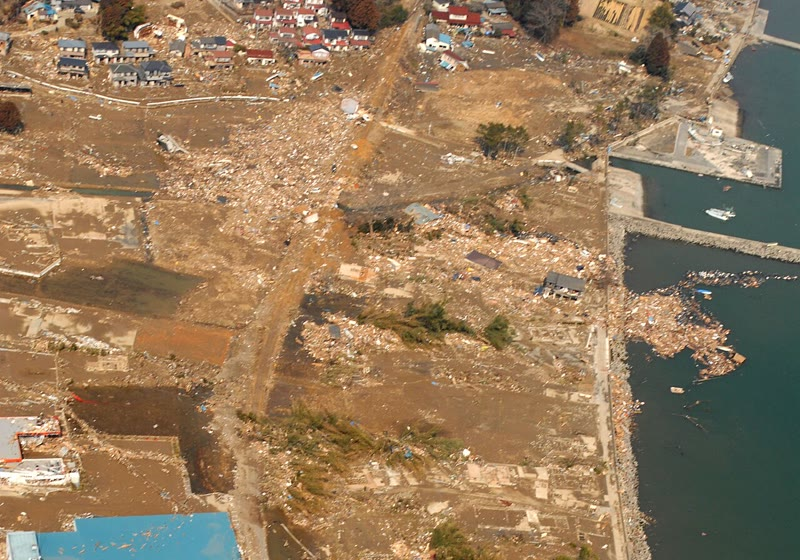
\includegraphics[width=0.78\linewidth]{images/book2/g11-usn-tsunami-kesennuma.jpg}

{\small Pelabuhan ikan Kesennuma, di pantai timur laut Jepang, dua hari setelah
tsunami 11~Maret 2011. Foto Dylan McCord, Angkatan Laut Amerika Serikat
(domain publik).}
\end{omfigure}
% ledger: photo:g11-tsunami

\section{Latihan}

\begin{exercise}[$\star$]\label{exo:g11:subduction-zones:1}
Definisikan \omterm{def:g11:subduction-zones:subduction}{subduksi} dan \omterm{def:g11:subduction-zones:subduction}{zona subduksi}. Jenis \omterm{def:g11:lithosphere-asthenosphere:lithosphere}{litosfer} apa yang tenggelam di \omterm{def:g11:subduction-zones:subduction}{zona
subduksi}, dan mengapa jenis itu?
\end{exercise}

\begin{exercise}[$\star$]\label{exo:g11:subduction-zones:2}
Dengan peta dunia gempa bumi menurut kedalaman: (1) sebutkan tiga wilayah dengan
gempa bumi yang lebih dalam daripada \qty{300}{km}; (2) di sisi palung yang mana
gempa-gempa bumi yang dalam terletak? (3) Di sepanjang Punggung Tengah Atlantik,
berapa kedalaman gempa-gempa buminya?
\end{exercise}

\begin{exercise}[$\star$]\label{exo:g11:subduction-zones:3}
Katalog itu memuat \num{7031} gempa bumi bermagnitudo 6 atau lebih, dengan
\qty{21}{\percent} lebih dalam daripada \qty{70}{km} dan \qty{6.9}{\percent}
lebih dalam daripada \qty{300}{km}. Berapa banyak gempa bumi itu pada setiap
kasus?
\end{exercise}

\begin{exercise}[$\star$]\label{exo:g11:subduction-zones:4}
Definisikan \omterm{def:g11:subduction-zones:eclogite}{sekis biru} dan \omterm{def:g11:subduction-zones:eclogite}{eklogit}. Apa kesamaan keduanya dengan basalt \omterm{def:g11:ocean-ridges:oceanic-lithosphere}{kerak
samudra}? Apa bedanya?
\end{exercise}

\begin{exercise}[$\star$]\label{exo:g11:subduction-zones:5}
Sebutkan bagian-bagian \omterm{def:g11:subduction-zones:subduction}{zona subduksi} secara berurutan, dari dasar samudra yang
bergerak ke arah palung sampai busur belakang, dengan menyatakan dalam satu baris
apa yang terjadi di masing-masing bagian.
\end{exercise}

\begin{exercise}[$\star\star$]\label{exo:g11:subduction-zones:6}
Pada penampang Andes, garis yang mengikuti gempa-gempa bumi melalui kedalaman
\qty{135}{km} pada jarak \qty{300}{km} dari palung dan kedalaman \qty{508}{km}
pada jarak \qty{800}{km}. Hitung kemiringan \omterm{def:g11:subduction-zones:slab}{lempengan} itu.
\end{exercise}

\begin{exercise}[$\star\star$]\label{exo:g11:subduction-zones:7}
Sebuah \omterm{def:g11:subduction-zones:slab}{lempengan} lurus bermula di palung dan miring \ang{45}. (1) Berapa
kedalamannya pada jarak \qty{300}{km} dari palung? (2) Pada jarak berapa dari
palung \omterm{def:g11:subduction-zones:slab}{lempengan} itu mencapai \qty{670}{km}? (3) Berapa panjang \omterm{def:g11:subduction-zones:slab}{lempengan} di
antara palung dan \qty{670}{km}?
\end{exercise}

\begin{exercise}[$\star\star$]\label{exo:g11:subduction-zones:8}
Kecepatan rata-rata lempeng-lempeng adalah, dalam milimeter setahun: Cocos 74.6,
Nazca 70.0, Pasifik 65.5, Australia 63.1, Laut Filipina 52.6 (dengan \omterm{def:g11:subduction-zones:slab}{lempengan});
Arab 47.6, Somalia 31.0, Nubia 29.2, Eurasia 22.8, Amerika Utara 19.8,
Antarktika 15.2, Karibia 14.9, Amerika Selatan 10.6 (tanpa \omterm{def:g11:subduction-zones:slab}{lempengan}).
(1) Hitung rata-rata setiap kelompok dan perbandingannya. (2) Apa yang
ditunjukkan hal ini tentang gaya yang menggerakkan lempeng?
\end{exercise}

\begin{exercise}[$\star\star$]\label{exo:g11:subduction-zones:9}
Pada tahun 2011 sesar di lepas pantai Jepang bergeser sampai sejauh 50 sampai
\qty{60}{m}. Lempeng Pasifik mendekat dengan kecepatan \qty{83}{mm} setahun.
(1) Berapa tahun gerak lempeng yang setara dengan pergeseran \qty{50}{m}, lalu
\qty{60}{m}? (2) Bandingkan dengan waktu sejak tahun 869, kemungkinan gempa bumi
sebelumnya yang sama besarnya.
\end{exercise}

\begin{exercise}[$\star\star$]\label{exo:g11:subduction-zones:10}
Dasar samudra yang mencapai Palung Jepang berumur sekitar 133 juta tahun, yang
mencapai Tonga sekitar 99, dan yang mencapai Andes sekitar 49. (1) Dengan hukum
pada \cref{ch:g11:ocean-ridges} ($2500 + 350\sqrt{t}$ untuk
$t \le 70$, $6400 - 3200\,e^{-t/62.8}$ di atasnya), tentukan kedalaman
masing-masing. (2) Manakah \omterm{def:g11:lithosphere-asthenosphere:lithosphere}{litosfer} yang paling dingin dan paling rapat?
\end{exercise}

\begin{exercise}[$\star\star$]\label{exo:g11:subduction-zones:11}
Basalt \omterm{def:g11:ocean-ridges:oceanic-lithosphere}{kerak samudra} mempunyai massa jenis sekitar \qty{2900}{kg/m^3}, mantel
di sekitar \omterm{def:g11:subduction-zones:slab}{lempengan} \qty{3380}{kg/m^3}, dan \omterm{def:g11:subduction-zones:eclogite}{eklogit} \qty{6}{\percent} lebih
rapat daripada mantel. (1) Tentukan massa jenis \omterm{def:g11:subduction-zones:eclogite}{eklogit}. (2) Sebesar berapa
persen massa jenis kerak naik ketika kerak itu berubah menjadi \omterm{def:g11:subduction-zones:eclogite}{eklogit}?
(3) Sebelum dan sesudahnya, apakah kerak itu lebih ringan atau lebih rapat
daripada mantel, dan berapa selisihnya?
\end{exercise}

\begin{exercise}[$\star\star\star$]\label{exo:g11:subduction-zones:12}
Kalor menyebar secara konduksi sejauh sekitar $\sqrt{\kappa t}$ dalam waktu $t$,
dengan $\kappa = \qty{1e-6}{m^2/s}$ untuk batuan. (1) Hitung jarak ini untuk 6
juta tahun ($1~\text{tahun} \approx \qty{3.16e7}{s}$). (2) Bandingkan dengan tebal
\omterm{def:g11:subduction-zones:slab}{lempengan}, sekitar \qty{100}{km}. (3) Jelaskan mengapa gempa bumi dapat terjadi
di dalam \omterm{def:g11:subduction-zones:slab}{lempengan} pada kedalaman \qty{600}{km} sementara mantel di sekitarnya
mengalir.
\end{exercise}
% ledger: england:kelvin (kappa 1e-6 m2/s)

\begin{exercise}[$\star\star\star$]\label{exo:g11:subduction-zones:13}
Di bawah Andes pada \ang{21}~LS, garis penampang mencapai \qty{670}{km} pada
jarak \qty{1017}{km} dari palung, dan lempeng-lempeng saling mendekat dengan
kecepatan \qty{64}{mm} setahun. (1) Taksirlah panjang \omterm{def:g11:subduction-zones:slab}{lempengan} dari palung
sampai \qty{670}{km}. (2) Berapa lama waktu yang diperlukan sepotong dasar
samudra untuk mencapai \qty{670}{km}? (3) Bandingkan dengan Tonga, tempat
perjalanan yang sama memerlukan sekitar 6 juta tahun.
\end{exercise}

\begin{exercise}[$\star\star\star$]\label{exo:g11:subduction-zones:14}
Ambillah \omterm{def:g11:subduction-zones:slab}{lempengan} setebal \qty{100}{km}, yang rata-rata \qty{36}{kg/m^3} lebih
rapat daripada mantel di sekitarnya, dan sepanjang \qty{1000}{km}, di bawah
sebuah palung. (1) Hitung kelebihan massa \omterm{def:g11:subduction-zones:slab}{lempengan} untuk setiap meter palung.
(2) Hitung beratnya, dengan $g = \qty{9.8}{m/s^2}$. (3) Mengapa gaya ini dapat
menarik seluruh lempeng?
\end{exercise}

\begin{exercise}[$\star\star\star$]\label{exo:g11:subduction-zones:15}
Di sepanjang Palung Tonga, model PB2002 memberikan laju saling mendekat sebesar
\qty{104}{mm} setahun pada \ang{23.6}~LS dan \qty{237}{mm} setahun pada
\ang{16.5}~LS. (1) Berapa jarak antara kedua titik itu, di sepanjang meridian
($\ang{1} \approx \qty{111}{km}$)? (2) Berapa laju itu bertambah per seratus
kilometer? (3) Lempeng Pasifik bergerak dengan kecepatan yang kira-kira sama di
kedua titik. Apa yang pasti sedang dilakukan sisi lain palung itu, yaitu busur
Tonga?
\end{exercise}

\section{Soal: Lempengan Tonga}

\begin{problem}[{Soal akhir pekan --- dari palung sampai \qty{670}{km}}]
\label{pb:g11:subduction-zones:1}
% values: tonga fit -23.568 + 0.91068 x; tonga_rate 168.0 mm/yr; tonga_age 98.8;
% x670 761.6; path 1014; time 6.04 Myr; tonga_maxdepth 670.8 (slab_sections.py);
% MKEA 69 mm/yr (plate_velocities.py); kappa england:kelvin; eclogite hacker03:eclogite
Di bawah Palung Tonga lempeng Pasifik tenggelam ke arah barat. Gunakan penampang
Tonga dalam bab ini, yang garisnya $z = -24 + 0.91\,x$ (keduanya dalam
kilometer, $x$ diukur dari palung ke arah busur).

\medskip
\noindent\textbf{Bagian I --- Penampang gempa bumi.}
\begin{enumerate}
  \item Berapa kedalaman gempa bumi yang paling dalam pada penampang itu?
  \item Mengapa tidak ada gempa bumi dalam di sisi samudra palung itu?
  \item Hitung kedalaman garis itu pada $x = 300$ dan $x = 700$, lalu
        kemiringan \omterm{def:g11:subduction-zones:slab}{lempengannya}.
  \item Pada jarak mendatar berapa dari palung \omterm{def:g11:subduction-zones:slab}{lempengan} itu berada pada
        kedalaman \qty{100}{km}? Dan pada kedalaman \qty{400}{km}?
  \item Garis itu melintas \qty{24}{km} di atas palung pada $x = 0$. Apa yang
        disampaikan hal ini tentang bentuk \omterm{def:g11:subduction-zones:slab}{lempengan} di dekat palung?
\end{enumerate}

\medskip
\noindent\textbf{Bagian II --- Saling mendekatnya lempeng.}
\begin{enumerate}[resume]
  \item Lempeng-lempeng saling mendekat melintasi palung dengan kecepatan sekitar
        \qty{168}{mm} setahun. Ubahlah ke sentimeter setahun dan kilometer per
        sejuta tahun.
  \item Lempeng Pasifik bergerak di atas Hawaii dengan kecepatan sekitar
        \qty{69}{mm} setahun. Berapa kali lebih cepat laju saling mendekat di
        Tonga?
  \item Dengan penjumlahan kecepatan relatif, jelaskan bagaimana laju saling
        mendekat itu dapat melampaui kecepatan lempeng Pasifik.
  \item Dasar yang mencapai palung berumur sekitar 99 juta tahun. Berapa
        kedalamannya (hukum eksponensial pada \cref{ch:g11:ocean-ridges})?
  \item Mengapa \omterm{def:g11:lithosphere-asthenosphere:lithosphere}{litosfer} seperti itu dapat tenggelam dengan sendirinya?
\end{enumerate}

\medskip
\noindent\textbf{Bagian III --- Turun sampai \qty{670}{km}.}
\begin{enumerate}[resume]
  \item Pada jarak mendatar berapa dari palung garis itu mencapai
        \qty{670}{km}?
  \item Taksirlah panjang \omterm{def:g11:subduction-zones:slab}{lempengan} dari palung sampai titik itu, dengan
        menganggapnya lurus.
  \item Berapa lama waktu yang diperlukan sepotong dasar samudra untuk menempuh
        panjang ini dengan kecepatan \qty{168}{mm} setahun?
  \item Berapa lama waktunya dengan \qty{69}{mm} setahun, kecepatan lempeng
        Pasifik di atas Hawaii?
  \item Dalam perjalanan itu, kerak \omterm{def:g11:subduction-zones:slab}{lempengan} berubah menjadi \omterm{def:g11:subduction-zones:eclogite}{eklogit}, yang
        \qty{6}{\percent} lebih rapat daripada mantel bermassa jenis
        \qty{3380}{kg/m^3}. Berapa massa jenisnya, dan apa yang diubah hal ini
        bagi \omterm{def:g11:subduction-zones:slab}{lempengan} itu?
\end{enumerate}

\medskip
\noindent\textbf{Bagian IV --- Lempengan dingin di dalam mantel yang panas.}
\begin{enumerate}[resume]
  \item Selama waktu pada pertanyaan~13, kalor menyebar secara konduksi sejauh
        sekitar $\sqrt{\kappa t}$, dengan $\kappa = \qty{1e-6}{m^2/s}$. Hitung
        jarak ini.
  \item Bandingkan dengan tebal \omterm{def:g11:subduction-zones:slab}{lempengan}, sekitar \qty{100}{km}. Apakah
        bagian dalam \omterm{def:g11:subduction-zones:slab}{lempengan} masih dingin ketika mencapai \qty{670}{km}?
  \item Mengapa hal ini menjelaskan gempa-gempa bumi pada kedalaman
        \qty{600}{km} dan lebih di bawah Tonga?
  \item Perubahan apa di mantel yang disingkapkan gelombang seismik di dekat
        \qty{670}{km} (\cref{ch:g11:seismic-structure})?
  \item Simpulkan: berapa lama waktu yang diperlukan dasar samudra Pasifik untuk
        turun dari Palung Tonga sampai \qty{670}{km}?
\end{enumerate}
\end{problem}
